\documentclass{article}%
\usepackage[T1]{fontenc}%
\usepackage[utf8]{inputenc}%
\usepackage{lmodern}%
\usepackage{textcomp}%
\usepackage{lastpage}%
\usepackage{geometry}%
\geometry{tmargin=1.5 in,lmargin=1.5in}%
\usepackage{amsmath}%
\usepackage{graphicx}%
%
\title{Método de Halley}%
%
\begin{document}%
\normalsize%
\maketitle%
\section{Desarrollo del problema}%
\label{sec:Desarrollodelproblema}%
\subsection{Datos}%
\label{subsec:Datos}%
\begin{alignat*}{2}%
f(x) = \frac{1}{2} - \cos{\left(x \right)}%
\end{alignat*}%
\begin{alignat*}{2}%
f'(x) = \sin{\left(x \right)}%
\end{alignat*}%
\begin{alignat*}{2}%
f''(x) = \cos{\left(x \right)}%
\end{alignat*}%
\begin{alignat*}{2}%
p0 = 0.0%
\end{alignat*}%
\begin{alignat*}{2}%
iter = 3.14%
\end{alignat*}%
\begin{alignat*}{2}%
\epsilon  = 1.0 \cdot 10^{-5}%
\end{alignat*}

%
\subsection{Validaciones}%
\label{subsec:Validaciones}%
\subsubsection{Evaluando la función en los intervalos}%
\label{ssubsec:Evaluandolafuncinenlosintervalos}%
Evaluando en funcion f(x) los intervalos {[}0.0, 3.14{]}: \newline%
%
\newline%
Evaluando el punto inicial en la función\newline%
%
\begin{alignat*}{2}%
f(p0) = -0.5%
\end{alignat*}%
\newline%
Evaluando la iteración o punto final en función\newline%
%
\begin{alignat*}{2}%
f(iter) = 1.4999987317275396%
\end{alignat*}

%
\subsubsection{Evaluando si existe la derivada}%
\label{ssubsec:Evaluandosiexisteladerivada}%
verificando derivada\newline%
%
\newline%
Evaluando la punto inicial en primera derivada\newline%
%
\begin{alignat*}{2}%
df(p0) = 0.0%
\end{alignat*}%
\newline%
Evaluando la iteración en primera derivada\newline%
%
\begin{alignat*}{2}%
df(iter) = 0.0015926529164868282%
\end{alignat*}%
Si tiene derivada, procedemos al desarrollo del problema...

%
\subsubsection{verificando la cota k en el intérvalo}%
\label{ssubsec:verificandolacotakenelintrvalo}%
\newline%
La cota para K en el intérvalo {[}0.0, 3.14{]} es: 3.14\newline%

%
\subsubsection{Evaluando iteraciones estimadas}%
\label{ssubsec:Evaluandoiteracionesestimadas}%
\newline%
Número de iteraciones estimadas: 11\newline%

%
\subsubsection{Evaluando Rapides de Convergencia}%
\label{ssubsec:EvaluandoRapidesdeConvergencia}%
\newline%
Rapidez de convergencia:%
\begin{alignat*}{2}%
O(3.14^n)%
\end{alignat*}

%
\subsection{Iteraciones}%
\label{subsec:Iteraciones}%
\subsubsection{Resultado de raíz aproximada del problema}%
\label{ssubsec:Resultadoderazaproximadadelproblema}%
Valor de raíz aproximada:%
\begin{alignat*}{2}%
1.02869976330546%
\end{alignat*}%
\subsubsection{Resultado de iteraciones de la función}%
\label{ssubsec:Resultadodeiteracionesdelafuncin}%
\begin{tabular}{c|c|c|c|c}%
\hline%
n&pn&f(pn)&f'(pn)&error\\%
0&0.0&{-}0.5&0.0&{-}\\%
1&0.5&{-}0.37758256189037276&0.479425538604203&0.5\\%
2&0.8729677361865782&{-}0.1425553842855335&0.7662392433996515&0.3729677361865782\\%
\hline%
\end{tabular}

%
\subsection{Visualización de grafica}%
\label{subsec:Visualizacindegrafica}%
\begin{alignat*}{2}%

Grafica para la función%
\end{alignat*}%
\begin{alignat*}{2}%
f(x) = \frac{1}{2} - \cos{\left(x \right)}%
\end{alignat*}%


\begin{figure}[h]%
\centering%
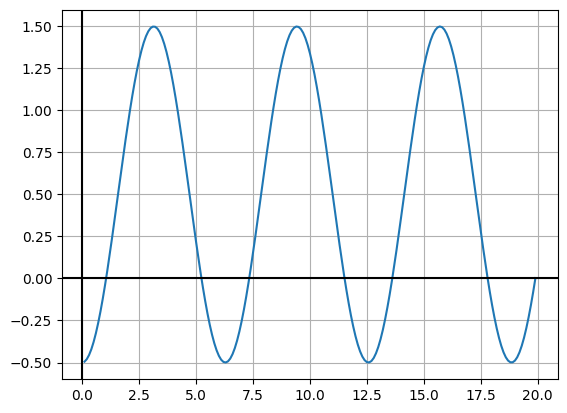
\includegraphics[width=250px]{ejemplo09_graph.png}%
\end{figure}

%
\end{document}